
\vspace{0.5 cm}
\begin{example} Calcular el volumen del sólido limitado por la esfera $x^2 + y^2 + z^2 \leq 1$ y el interior del cono $x^2 + y^2 \leq z^2$.
\end{example}

\vspace{0.3cm}
\textbf{Soluci\'on:}
\bigskip
\textbf{Análisis de la región y simetría}

La región $W \subseteq \mathbb{R}^3$ está definida por el interior de la esfera de radio 1 y el interior del cono. Matemáticamente, lo expresamos como:
\[
    W = \{ (x,y,z) \in \mathbb{R}^3 \mid x^2 + y^2 + z^2 \leq 1, \ x^2 + y^2 \leq z^2 \}
\]

\begin{figure}[htbp]
    \centering
    % Llamamos al archivo con el código TikZ extraído
    
    \centering
    \tikzsetnextfilename{ejercicio28_figura} 
    
    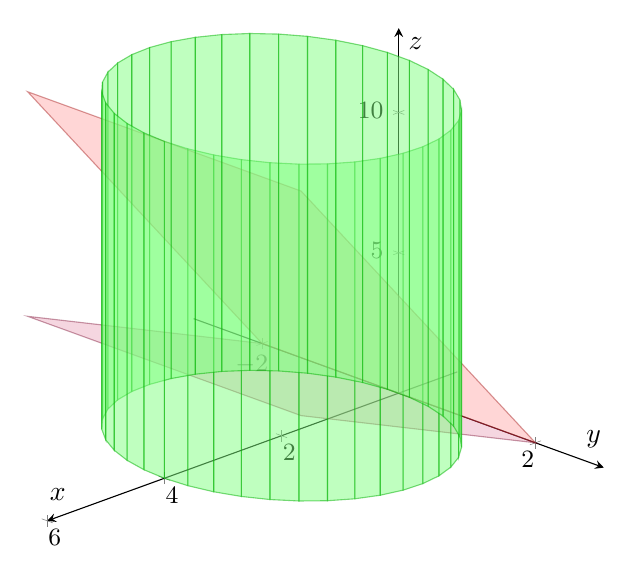
\begin{tikzpicture}
        \begin{axis}[
            view={135}{30}, % Ajustado para ver bien la inclinación de los planos
            width=12cm,
            height=10cm,
            grid=major,
            xmin=-1, xmax=6,
            ymin=-3, ymax=3,
            zmin=0, zmax=13,
            xlabel={$x$},
            ylabel={$y$},
            zlabel={$z$},
            axis lines=center,
            ticklabel style={font=\small},
        ]

        % Plano g: z = x (Violeta)
        \addplot3[
            surf,
            domain=0:4,
            y domain=-2:2,
            samples=2,
            color=purple!40,
            opacity=0.4,
            faceted color=purple!60!black,
        ] {x};

        % Plano h: z = 3x (Rojo)
        \addplot3[
            surf,
            domain=0:4,
            y domain=-2:2,
            samples=2,
            color=red!40,
            opacity=0.4,
            faceted color=red!60!black,
        ] {3*x};

        % Cilindro f: (x-2)^2 + y^2 = 4 (Verde)
        % Parametrización: x = 2 + 2*cos(t), y = 2*sin(t)
        \addplot3[
            surf,
            domain=0:360, % ángulo t
            y domain=0:12, % altura z (hasta el máximo de 3x)
            samples=40,
            samples y=2,
            color=green!50,
            opacity=0.5,
            faceted color=green!70!black,
        ]
        ({2 + 2*cos(x)}, {2*sin(x)}, {y});

        \end{axis}
    \end{tikzpicture}
    \caption{Representación de la región pedida.  \href{https://www.geogebra.org/m/uhgycge3}{Ver en GeoGebra}}
 
    \label{fig:Ejemplo 8.2.5}
\end{figure}

Observamos que el sólido es simétrico respecto al plano $xy$ ($z=0$). Para simplificar el cálculo, trabajaremos únicamente con la mitad superior del sólido (donde $z \geq 0$), a la cual llamaremos $W_s$:
\[
    W_s = \{ (x,y,z) \in \mathbb{R}^3 \mid x^2 + y^2 + z^2 \leq 1, \ x^2 + y^2 \leq z^2, \ z \geq 0 \}
\]

Gracias a dicha simetría podemos calcular el volumen total sabiendo que es el doble del volumen de la región superior: $\text{Vol}(W) = 2 \, \text{Vol}(W_s)$. 

A su vez, de acuerdo con la definición~\ref{def:vol_solido}, el volumen de un sólido se calcula mediante la integral triple de la función constante $1$. Combinando ambas ideas, planteamos:
\[
    \text{Vol}(W) = 2 \iiint_{W_s} 1 \, dV
\]

\textbf{Cambio de variables a coordenadas esféricas \footnote{El planteo completo de este sistema de coordenadas y la deducción de su jacobiano se encuentran disponibles en la sección~\ref{sec:coordenadas_esfericas}.}}  

Para resolver la integral, aplicamos el Teorema~\ref{teo:cambio_variable} utilizando la transformación a esféricas:
\begin{align*}
    x &= \rho \sin \phi \cos \theta \\
    y &= \rho \sin \phi \sin \theta \\
    z &= \rho \cos \phi
\end{align*}

Tal como se demuestra en el ejemplo~\ref{ej:jacobiano_esferico}, el valor absoluto del determinante jacobiano es $|J_{\mathbf{T}}| = \rho^2 \sin \phi$.

\vspace{0.3cm}
\textbf{Nuevos parámetros en $W^*$}

Definimos el conjunto $W^*$ analizando las restricciones sobre nuestra región $W_s$:

\textbf{Rango de $\rho$:} La esfera $x^2 + y^2 + z^2 \leq 1$ define el radio máximo. En esféricas $\rho^2 \leq 1$, por lo tanto $0 \leq \rho \leq 1$.

\textbf{Rango de $\theta$:} El sólido es de revolución completa alrededor del eje $z$. Por lo tanto $0 \leq \theta \leq 2\pi$.

\textbf{Rango de $\phi$ (Triángulo de Intersección):} Buscamos el ángulo máximo donde el cono intercepta a la esfera. Al igualar $x^2 + y^2 = z^2$ con $x^2 + y^2 + z^2 = 1$, obtenemos $2z^2 = 1 \implies z = \frac{1}{\sqrt{2}}$. Este valor de $z$ es nuestro cateto adyacente. El radio del cono en esa altura es el cateto opuesto, que también vale $\sqrt{x^2+y^2} = z = \frac{1}{\sqrt{2}}$.

\begin{figure}[htbp]
    \centering
    % Llamamos al archivo con el código TikZ extraído
    
    \centering
    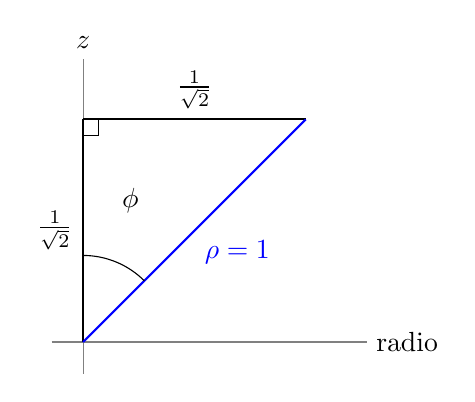
\begin{tikzpicture}[scale=4]
        % Coordenadas
        \coordinate (O) at (0,0); 
        \coordinate (A) at (0,{1/sqrt(2)}); 
        \coordinate (B) at ({1/sqrt(2)},{1/sqrt(2)}); 

        % Ejes tenues
        \draw[gray] (-0.1,0) -- (0.9,0) node[right, black] {radio};
        \draw[gray] (0,-0.1) -- (0,0.9) node[above, black] {$z$};

        % Dibujo del triángulo
        \draw[thick] (O) -- (A) node[midway, left] {$\frac{1}{\sqrt{2}}$}; 
        \draw[thick] (A) -- (B) node[midway, above] {$\frac{1}{\sqrt{2}}$}; 
        \draw[thick, blue] (O) -- (B) node[midway, below right] {$\rho=1$}; 

        % Ángulo recto
        \draw (A) ++(0,-0.05) -- ++(0.05,0) -- ++(0,0.05);

        % Arco de phi interno (Solucionado: dibujado a mano sin depender de librerías)
        \draw (0, 0.275) arc (90:45:0.275);
        \node at (0.15, 0.45) {$\phi$};
    \end{tikzpicture}
 
    \label{fig:triangulo de interseccion}
\end{figure}

Planteamos la relación trigonométrica según el esquema anterior:
\[
    \tan(\phi) = \frac{\text{Cat. Opuesto}}{\text{Cat. Adyacente}} = \frac{1/\sqrt{2}}{1/\sqrt{2}} = 1 \implies \phi = \arctan(1) = \frac{\pi}{4}
\]
    
Como el ángulo nace en el eje $z$ (que es positivo en $W_s$), los límites son $0 \leq \phi \leq \frac{\pi}{4}$.

\vspace{0.3cm}
\textbf{Cálculo del Volumen}

Planteamos primero la integral triple para $W_s$. Debido a que los límites son constantes, podemos separar la expresión en el producto de tres integrales simples:

\[
    \text{Vol}(W_s) = \int_{0}^{2\pi} \int_{0}^{\pi/4} \int_{0}^{1} \rho^2 \sin \phi \, d\rho \, d\phi \, d\theta = \int_{0}^{2\pi} d\theta \int_{0}^{\pi/4} \sin \phi \, d\phi \int_{0}^{1} \rho^2 \, d\rho
\]

Calculamos cada parte de forma independiente:
\[ \int_{0}^{1} \rho^2 \, d\rho = \left[ \frac{\rho^3}{3} \right]_{0}^{1} = \frac{1}{3} \]
\[ \int_{0}^{\pi/4} \sin \phi \, d\phi = \left[ -\cos \phi \right]_{0}^{\pi/4} = -\frac{\sqrt{2}}{2} - (-1) = 1 - \frac{\sqrt{2}}{2} \]
\[ \int_{0}^{2\pi} d\theta = \left[ \theta \right]_{0}^{2\pi} = 2\pi \]

Combinando los resultados parciales y multiplicando por 2 (por la simetría original):
\begin{align*}
    \text{Vol}(W) &= 2 \, \text{Vol}(W_s) \\
    &= 2 \left( 2\pi \right) \left( 1 - \frac{\sqrt{2}}{2} \right) \left( \frac{1}{3} \right) \\
    &= \frac{4\pi}{3} \left( 1 - \frac{\sqrt{2}}{2} \right)
\end{align*}